\documentclass[tikz]{standalone}

\begin{document}
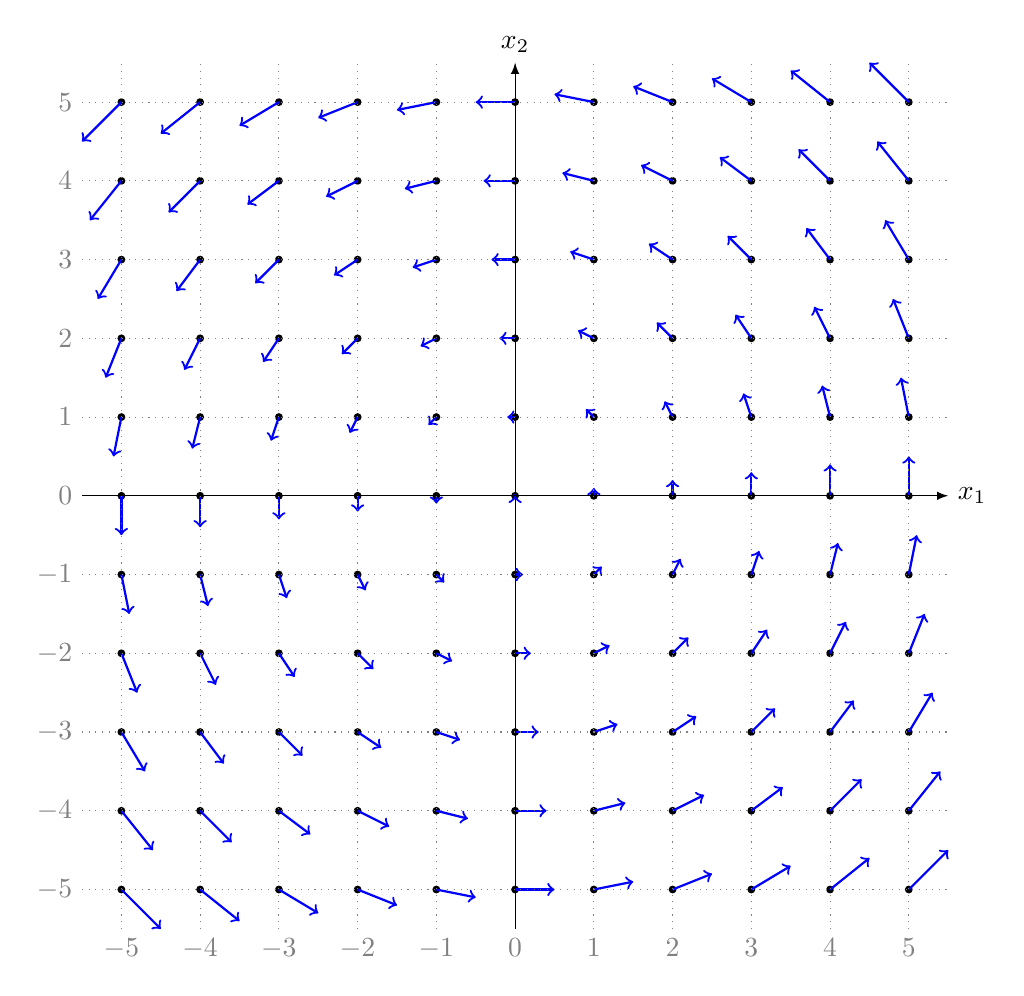
\begin{tikzpicture}
  \foreach \x in {-5,-4, ..., 5}
  {
    \foreach \y in {-5,-4, ..., 5}
    {
      \fill (\x, \y) circle (0.05cm);
      \draw[->,=>stealth,blue,thick]
        (\x,\y) -- (\x -0.1*\y, \y + 0.1*\x);
    }
  }
  \foreach \x in {-5,-4, ..., 5}
  {
    \draw[gray,dotted] (-5.5,\x) -- (5.5, \x);
    \draw[gray,dotted] (\x,-5.5) -- (\x, 5.5);
    \node[below, gray] at (\x,-5.5) {\(\x\)};
    \node[left, gray] at (-5.5,\x) {\(\x\)};
  }
  \draw[-latex] (-5.5,0)--(5.5,0) node [right] {\(x_1\)};
  \draw[-latex] (0,-5.5)--(0,5.5) node [above] {\(x_2\)};

\end{tikzpicture}
\end{document}
